\chapter{Grandezze vettoriali e forze}

Fino a qui abbiamo trattato grandezze che, per essere assegnate, richiedono soltanto un numero e un'unità di misura: una massa di $\SI{3}{\kilo\gram}$, un intervallo di $\SI{12}{\second}$, un volume di $\SI{2}{\liter}$. In questo capitolo incontreremo grandezze di tipo diverso, per le quali il solo numero non basta: occorre indicare anche una \textit{direzione}. Sono le grandezze vettoriali, e la prima che studieremo è lo spostamento. Introdurremo le regole per sommarle e sottrarle, e poi le applicheremo alle forze.

\section{Grandezze scalari e vettoriali}

Immaginiamo di dare a qualcuno l'indicazione: ``spostati di $\SI{5}{\meter}$''. L'informazione è incompleta: in quale direzione? in avanti o indietro? Per descrivere completamente uno spostamento dobbiamo dire \textbf{di quanto} ci si sposta (per esempio $\SI{5}{\meter}$), lungo \textbf{quale retta} (per esempio la direzione Est--Ovest) e in \textbf{quale dei due versi} (verso Est). Lo spostamento è l'esempio tipico di grandezza vettoriale.

\begin{definizione}
Una grandezza si dice \textbf{scalare} quando è completamente determinata da un numero (con la sua unità di misura). Sono scalari la massa, il tempo, la temperatura, la lunghezza, l'area, il volume, la densità.
\end{definizione}

\begin{definizione}
Una grandezza si dice \textbf{vettoriale} quando, per essere assegnata, richiede tre informazioni: un \textbf{modulo} (o intensità), una \textbf{direzione} e un \textbf{verso}. Sono vettoriali lo spostamento, la velocità, l'accelerazione, la forza.
\end{definizione}

\subsection{Rappresentazione di un vettore}
Una grandezza vettoriale si associa a un ente matematico chiamato \textbf{vettore}, che si disegna come un \textbf{segmento orientato}, cioè una freccia (figura~\ref{fig:vettore}):
\begin{itemize}
\item la \textbf{lunghezza} della freccia, in una scala scelta, rappresenta il \textbf{modulo};
\item la \textbf{retta} su cui giace la freccia è la \textbf{direzione};
\item la \textbf{punta} della freccia indica il \textbf{verso}.
\end{itemize}
I vettori si indicano con una lettera sormontata da una freccetta, $\vec{v}$, oppure con le due lettere degli estremi del segmento orientato, $\vec{AB}$ (dove $A$ è la coda e $B$ la punta). Il modulo si scrive $|\vec{v}|$ oppure, più semplicemente, con la lettera senza freccia, $v$.

\begin{figure}[h!]
\centering
\begin{tikzpicture}[scale=1]
\draw[->,very thick,ocre] (0,0) -- (4.2,1.4) node[midway,above,sloped]{modulo};
\draw[dashed,gray] (-0.6,-0.2) -- (5.1,1.7) node[right,black]{direzione};
\node[ocre] at (4.35,1.15) {verso};
\fill (0,0) circle (1.5pt) node[below left]{$A$};
\node at (2,-0.9) {$\vec{v}=\vec{AB}$};
\end{tikzpicture}
\caption{Un vettore: la lunghezza dà il modulo, la retta la direzione, la punta il verso.}
\label{fig:vettore}
\end{figure}

\begin{remark}
Il modulo di un vettore è sempre un numero \textbf{positivo} (o nullo): è una lunghezza, un'intensità, e non ha senso che sia negativo. Il ``segno'' di una grandezza vettoriale è portato dal verso, non dal modulo.
\end{remark}

\subsection{Vettore nullo e vettore opposto}
Il \textbf{vettore nullo} $\vec{0}$ ha modulo zero; direzione e verso sono indeterminati. Corrisponde, per lo spostamento, al non essersi mossi.

Dato un vettore $\vec{v}$, il suo \textbf{opposto} $-\vec{v}$ ha lo \textbf{stesso modulo} e la \textbf{stessa direzione}, ma \textbf{verso contrario} (figura~\ref{fig:opposto}). Per lo spostamento, $-\vec{v}$ è il ``tornare indietro'' lungo lo stesso tragitto.

\begin{figure}[h!]
\centering
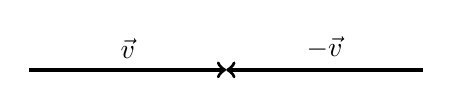
\begin{tikzpicture}[scale=1]
\draw[->,very thick] (0,0) -- (2.5,0) node[midway,above]{$\vec{v}$};
\draw[->,very thick] (5,0) -- (2.5,0) node[midway,above]{$-\vec{v}$};
\end{tikzpicture}
\caption{Un vettore e il suo opposto: stesso modulo e direzione, verso contrario.}
\label{fig:opposto}
\end{figure}

\section{Operazioni con i vettori}\label{sec:operazioni-vettori}

\subsection{Somma di vettori sulla stessa retta}
Se due spostamenti avvengono lungo la stessa retta, la somma si riduce a un calcolo con i numeri, tenendo conto del verso:
\begin{itemize}
\item se hanno lo \textbf{stesso verso}, i moduli si \textbf{sommano};
\item se hanno \textbf{verso opposto}, i moduli si \textbf{sottraggono} e il verso del risultante è quello del vettore di modulo maggiore.
\end{itemize}

\begin{figure}[h!]
\centering
\begin{tikzpicture}[scale=0.85]
% stesso verso
\draw[->,thick] (0,0.35) -- (2,0.35) node[midway,above]{\small $\vec{a}$};
\draw[->,thick] (2,0.35) -- (3,0.35) node[midway,above]{\small $\vec{b}$};
\draw[->,very thick,ocre] (0,-0.35) -- (3,-0.35) node[midway,below]{\small $\vec{a}+\vec{b}=\SI{11}{m}$};
\node[align=center] at (1.5,-1.3) {\scriptsize stesso verso};
\begin{scope}[xshift=6.5cm]
% verso opposto
\draw[->,thick] (0,0.35) -- (3,0.35) node[midway,above]{\small $\vec{a}$};
\draw[->,thick] (3,-0.05) -- (2,-0.05) node[midway,below]{\small $\vec{b}$};
\draw[->,very thick,ocre] (0,-0.75) -- (2,-0.75) node[midway,below]{\small $\vec{a}+\vec{b}=\SI{5}{m}$};
\node[align=center] at (1.5,-1.7) {\scriptsize verso opposto};
\end{scope}
\end{tikzpicture}
\caption{Somma di due vettori sulla stessa retta: stesso verso (a sinistra) e verso opposto (a destra).}
\label{fig:sommaretta}
\end{figure}

\subsection{Metodo punta-coda}
Quando i due vettori non sono sulla stessa retta, si usa il \textbf{metodo punta-coda}: si trasla il secondo vettore, senza cambiarne modulo, direzione e verso, in modo che la sua coda coincida con la punta del primo. Il vettore \textbf{risultante} è il segmento orientato che va dalla coda del primo alla punta del secondo (figura~\ref{fig:puntacoda}).

Lo stesso metodo si estende a più vettori: si dispongono uno di seguito all'altro e il risultante chiude la spezzata, dalla coda del primo alla punta dell'ultimo.

\begin{figure}[h!]
\centering
\begin{tikzpicture}[scale=1]
\coordinate (O) at (0,0);
\coordinate (A) at (3,0.6);
\coordinate (B) at (4,2.4);
\draw[->,thick] (O) -- (A) node[midway,below right]{$\vec{a}$};
\draw[->,thick] (A) -- (B) node[midway,right]{$\vec{b}$};
\draw[->,very thick,ocre] (O) -- (B) node[midway,above left]{$\vec{a}+\vec{b}$};
\end{tikzpicture}
\caption{Metodo punta-coda per la somma di due vettori.}
\label{fig:puntacoda}
\end{figure}

\subsection{Regola del parallelogramma}
Se i due vettori sono applicati nello stesso punto, si può usare la \textbf{regola del parallelogramma}, equivalente al metodo punta-coda: si costruisce il parallelogramma che ha per lati i due vettori, e la \textbf{diagonale} uscente dal punto comune è il vettore risultante (figura~\ref{fig:parallelogramma}).

\begin{figure}[h!]
\centering
\begin{tikzpicture}[scale=1]
\coordinate (O) at (0,0);
\coordinate (A) at (3,0);
\coordinate (B) at (1.2,2);
\coordinate (C) at (4.2,2);
\draw[->,thick] (O) -- (A) node[midway,below]{$\vec{a}$};
\draw[->,thick] (O) -- (B) node[midway,above left]{$\vec{b}$};
\draw[dashed,gray] (A) -- (C) -- (B);
\draw[->,very thick,ocre] (O) -- (C) node[midway,above right]{$\vec{a}+\vec{b}$};
\end{tikzpicture}
\caption{Regola del parallelogramma.}
\label{fig:parallelogramma}
\end{figure}

\begin{remark}
La somma di vettori è \textbf{commutativa}: $\vec{a}+\vec{b}=\vec{b}+\vec{a}$. Il modulo del risultante \textbf{non} è, in generale, la somma dei moduli: dipende dall'angolo tra i due vettori. È uguale alla somma dei moduli solo se i vettori hanno lo stesso verso; è uguale alla differenza se hanno verso opposto.
\end{remark}

\subsection{Differenza di vettori}
La differenza $\vec{a}-\vec{b}$ si definisce come la somma del primo con l'opposto del secondo:
\[
\vec{a}-\vec{b}=\vec{a}+(-\vec{b}).
\]
In pratica si ribalta $\vec{b}$ e lo si somma ad $\vec{a}$ con il metodo punta-coda (figura~\ref{fig:differenza}).

\begin{figure}[h!]
\centering
\begin{tikzpicture}[scale=1]
\coordinate (O) at (0,0);
\coordinate (A) at (3,0.4);
\coordinate (mB) at (3.8,-1.6);
\draw[->,thick] (O) -- (A) node[midway,above]{$\vec{a}$};
\draw[->,thick] (A) -- (mB) node[midway,right]{$-\vec{b}$};
\draw[->,very thick,ocre] (O) -- (mB) node[midway,below left]{$\vec{a}-\vec{b}$};
\end{tikzpicture}
\caption{Differenza di due vettori: $\vec{a}-\vec{b}=\vec{a}+(-\vec{b})$.}
\label{fig:differenza}
\end{figure}

\subsection{Moltiplicazione di un vettore per un numero}
Moltiplicando un vettore $\vec{v}$ per un numero $k$ (uno scalare) si ottiene un nuovo vettore $k\,\vec{v}$:
\begin{itemize}
\item di modulo $|k|\cdot v$;
\item con la \textbf{stessa direzione} di $\vec{v}$;
\item con lo \textbf{stesso verso} se $k>0$, con verso \textbf{opposto} se $k<0$.
\end{itemize}
Per esempio $3\vec{v}$ è tre volte più lungo di $\vec{v}$ e con lo stesso verso; $-2\vec{v}$ è due volte più lungo e con verso opposto.

\subsection{Somma di due vettori perpendicolari}
Un caso particolare importante è la somma di due vettori \textbf{perpendicolari} tra loro. Poiché il metodo punta-coda forma in questo caso un triangolo rettangolo, il modulo del risultante si ottiene con il \textbf{teorema di Pitagora} (figura~\ref{fig:perpendicolari}):
\[
\colorboxed{ocre}{\;|\vec{a}+\vec{b}| = \sqrt{a^2+b^2}\;}
\]
La direzione del risultante si individua con l'angolo $\theta$ che esso forma con uno dei due vettori: $\tan\theta = \dfrac{\text{cateto opposto}}{\text{cateto adiacente}}$.

\begin{figure}[h!]
\centering
\begin{tikzpicture}[scale=0.8]
\coordinate (O) at (0,0);
\coordinate (A) at (4,0);
\coordinate (B) at (4,3);
\draw[->,thick] (O) -- (A) node[midway,below]{$\vec{a}$};
\draw[->,thick] (A) -- (B) node[midway,right]{$\vec{b}$};
\draw[->,very thick,ocre] (O) -- (B) node[midway,above left]{$\vec{a}+\vec{b}$};
\draw (0.5,0) arc (0:36.87:0.5); \node at (0.95,0.25){\small $\theta$};
\draw (3.75,0) rectangle (4,0.25);
\end{tikzpicture}
\caption{Somma di due vettori perpendicolari: il modulo si trova con Pitagora.}
\label{fig:perpendicolari}
\end{figure}

\begin{testexample}[\thetcbcounter \, Spostamento risultante]
Un'escursionista percorre $\SI{40}{\meter}$ verso Est e poi $\SI{30}{\meter}$ verso Nord. Qual è il suo spostamento risultante rispetto al punto di partenza?

I due spostamenti sono perpendicolari, quindi il modulo del risultante è:
\[
s = \sqrt{(\SI{40}{\meter})^2 + (\SI{30}{\meter})^2} = \sqrt{\SI{2500}{\meter\squared}} = \SI{50}{\meter}.
\]
La direzione forma con l'Est un angolo $\theta$ tale che $\tan\theta = \dfrac{30}{40} = 0,75$, da cui $\theta \approx 37^\circ$. Lo spostamento risultante è dunque di $\SI{50}{\meter}$, in direzione Nord-Est a circa $37^\circ$ dall'Est.
\end{testexample}

\begin{testexample}[\thetcbcounter \, Due spostamenti collineari]
Un carrello si sposta di $\SI{8}{\meter}$ verso destra, poi di $\SI{3}{\meter}$ ancora verso destra: lo spostamento risultante ha modulo $\SI{8}{\meter}+\SI{3}{\meter}=\SI{11}{\meter}$, verso destra. Se invece il secondo spostamento fosse di $\SI{3}{\meter}$ verso \emph{sinistra}, il risultante avrebbe modulo $\SI{8}{\meter}-\SI{3}{\meter}=\SI{5}{\meter}$, verso destra.
\end{testexample}

\subsection{Esercizi}

\begin{esercizio}
Classifica le seguenti grandezze come scalari o vettoriali: massa, velocità, temperatura, forza, tempo, spostamento, volume, accelerazione.\\
\risp{scalari: massa, temperatura, tempo, volume; vettoriali: velocità, forza, spostamento, accelerazione}
\end{esercizio}

\begin{esercizio}
Due vettori giacciono sulla stessa retta: $\vec{a}$ ha modulo $\SI{12}{\newton}$ ed è diretto verso Est, $\vec{b}$ ha modulo $\SI{5}{\newton}$ ed è diretto verso Ovest. Determina modulo e verso di $\vec{a}+\vec{b}$ e di $\vec{a}-\vec{b}$.\\
\risp{$\vec{a}+\vec{b}:\ \SI{7}{\newton}\ \text{verso Est}\ ;\quad \vec{a}-\vec{b}:\ \SI{17}{\newton}\ \text{verso Est}$}
\end{esercizio}

\begin{esercizio}
Un'imbarcazione compie uno spostamento di $\SI{60}{\meter}$ verso Nord e uno di $\SI{80}{\meter}$ verso Est. Calcola il modulo dello spostamento risultante e l'angolo che esso forma con la direzione Nord.\\
\risp{$s=\SI{100}{\meter}\ ;\quad \theta \approx 53^\circ$}
\end{esercizio}

\begin{esercizio}
Un vettore $\vec{v}$ ha modulo $\SI{3}{\meter\per\second}$. Qual è il modulo del vettore $-2\,\vec{v}$? E il suo verso rispetto a $\vec{v}$?\\
\risp{$\text{modulo}\ \SI{6}{\meter\per\second}\ ;\quad \text{verso opposto a } \vec{v}$}
\end{esercizio}

\begin{esercizio}
Su un punto agiscono due forze perpendicolari, di moduli $\SI{9}{\newton}$ e $\SI{12}{\newton}$. Determina il modulo della forza risultante.\\
\risp{$R=\SI{15}{\newton}$}
\end{esercizio}

\begin{esercizio}
Disegna su un foglio a quadretti due vettori $\vec{a}$ (orizzontale, verso destra, 4 quadretti) e $\vec{b}$ (verticale, verso l'alto, 3 quadretti) applicati nello stesso punto. Trova graficamente $\vec{a}+\vec{b}$ con la regola del parallelogramma e verifica, contando i quadretti e usando Pitagora, che il modulo del risultante è 5 quadretti.
\end{esercizio}


\section{La scomposizione di un vettore}\label{sec:scomposizione}

L'operazione inversa della somma si chiama \textbf{scomposizione}: dato un vettore $\vec{v}$, si cercano due vettori la cui somma sia $\vec{v}$. Il problema ha infinite soluzioni, ma quasi sempre conviene scegliere due direzioni \textbf{perpendicolari} tra loro, di solito quelle di un sistema di assi cartesiani $x$ e $y$.

\subsection{Vettori componenti e componenti}
Fissati gli assi, si tracciano dalla punta di $\vec{v}$ le perpendicolari ai due assi. Si ottengono così due vettori, $\vec{v}_x$ lungo l'asse $x$ e $\vec{v}_y$ lungo l'asse $y$, detti \textbf{vettori componenti} di $\vec{v}$, tali che (figura~\ref{fig:scomposizione}):
\[
\vec{v} = \vec{v}_x + \vec{v}_y .
\]

\begin{figure}[h!]
\centering
\begin{tikzpicture}[scale=1]
\draw[->] (-0.5,0) -- (5,0) node[right]{$x$};
\draw[->] (0,-0.5) -- (0,3.4) node[above]{$y$};
\coordinate (P) at (4,2.6);
\draw[->,very thick,ocre] (0,0) -- (P) node[midway,above left]{$\vec{v}$};
\draw[->,thick,blue!60!black] (0,0) -- (4,0) node[midway,below]{$\vec{v}_x$};
\draw[->,thick,blue!60!black] (0,0) -- (0,2.6) node[midway,left]{$\vec{v}_y$};
\draw[dashed,gray] (4,0) -- (P) -- (0,2.6);
\draw (0.55,0) arc (0:33:0.55); \node at (0.95,0.22){\small $\alpha$};
\end{tikzpicture}
\caption{Scomposizione di un vettore lungo due assi perpendicolari.}
\label{fig:scomposizione}
\end{figure}

Spesso è più comodo lavorare con numeri anziché con vettori. Si introducono allora le \textbf{componenti} $v_x$ e $v_y$: sono numeri (scalari) con segno, il cui valore assoluto è il modulo del corrispondente vettore componente, e il cui segno è positivo se il vettore componente è concorde con il verso dell'asse, negativo se è discorde. Le componenti si scrivono senza freccia.

Poiché $\vec{v}$, $\vec{v}_x$ e $\vec{v}_y$ formano un triangolo rettangolo di cui $\vec{v}$ è l'ipotenusa, vale il \textbf{teorema di Pitagora}:
\[
\colorboxed{ocre}{\; v = \sqrt{v_x^2 + v_y^2}\; }
\]

\subsection{Calcolo delle componenti}
Se si conosce l'angolo $\alpha$ che $\vec{v}$ forma con l'asse $x$:
\begin{itemize}
\item per $\alpha = 45^\circ$ le due componenti sono uguali e valgono $v_x = v_y = \dfrac{v}{\sqrt{2}} \approx 0,71\,v$;
\item per $\alpha = 30^\circ$ o $\alpha = 60^\circ$ si usa il triangolo rettangolo con angoli $30^\circ$--$60^\circ$--$90^\circ$, in cui il cateto opposto all'angolo di $30^\circ$ è metà dell'ipotenusa;
\item per un angolo qualunque, quando conoscerete la trigonometria, si userà $v_x = v\cos\alpha$ e $v_y = v\sin\alpha$.
\end{itemize}

\begin{testexample}[\thetcbcounter \, Scomposizione di uno spostamento]
Uno spostamento $\vec{v}$ ha modulo $\SI{10}{\meter}$ e forma un angolo di $30^\circ$ con l'asse $x$. La componente lungo $y$ è metà del modulo: $v_y = \SI{5}{\meter}$. La componente lungo $x$ si ricava con Pitagora:
\[
v_x = \sqrt{v^2 - v_y^2} = \sqrt{(\SI{10}{\meter})^2 - (\SI{5}{\meter})^2} = \sqrt{\SI{75}{\meter\squared}} \approx \SI{8,7}{\meter}.
\]
\end{testexample}

\subsection{Esercizi}

\begin{esercizio}
Un vettore ha componenti $v_x = \SI{9}{\meter}$ e $v_y = \SI{12}{\meter}$. Calcola il suo modulo.\\
\risp{$v = \SI{15}{\meter}$}
\end{esercizio}

\begin{esercizio}
Uno spostamento di modulo $\SI{20}{\meter}$ forma un angolo di $60^\circ$ con l'asse $x$. Determina le due componenti (suggerimento: qual è metà dell'ipotenusa?).\\
\risp{$v_x = \SI{10}{\meter}\ ;\quad v_y \approx \SI{17,3}{\meter}$}
\end{esercizio}

\begin{esercizio}
Una forza di modulo $\SI{50}{\newton}$ è inclinata di $45^\circ$ rispetto all'orizzontale. Quanto valgono le sue componenti orizzontale e verticale?\\
\risp{$F_x = F_y = \dfrac{50}{\sqrt{2}}\,\si{\newton} \approx \SI{35}{\newton}$}
\end{esercizio}


\section{Le forze}

Nel linguaggio comune usiamo spesso la parola ``forza'', ma darne una definizione precisa non è semplice. Ci accorgiamo che è in gioco una forza quando osserviamo i suoi \textbf{effetti}: serve una forza per tenere fermo un aquilone che vorrebbe volare via, per sollevare uno zaino, per deformare una molla o una gomma da cancellare. Possiamo quindi dire:

\begin{definizione}
Una \textbf{forza} è tutto ciò che produce una variazione del moto (un'accelerazione) oppure una deformazione di un corpo.
\end{definizione}

\subsection{Forze di contatto e forze a distanza}
Negli esempi visti sopra c'è sempre un contatto tra chi esercita la forza e il corpo su cui agisce: si parla di \textbf{forze di contatto}. Esistono però anche \textbf{forze a distanza}, che agiscono senza contatto: la forza con cui una calamita attira un chiodo di ferro, la forza elettrica tra oggetti carichi, e soprattutto la forza di gravità con cui la Terra attira tutti i corpi.

\subsection{La forza come vettore}
La forza è una grandezza \textbf{vettoriale}: per assegnarla occorrono un modulo (l'intensità), una direzione (la \textbf{retta d'azione} della forza) e un verso. Va inoltre specificato il \textbf{punto di applicazione}, cioè il punto del corpo su cui la forza agisce (figura~\ref{fig:forzavettore}).

\begin{figure}[h!]
\centering
\begin{tikzpicture}[scale=1]
\fill[gray!25] (0,0) rectangle (1.6,1);
\draw (0,0) rectangle (1.6,1);
\fill (1.6,0.5) circle (1.5pt) node[below right]{\small punto di applicazione};
\draw[->,very thick,ocre] (1.6,0.5) -- (4.3,0.5) node[midway,above]{$\vec{F}$};
\draw[dashed,gray] (-0.4,0.5) -- (5,0.5) node[right,black]{\small retta d'azione};
\end{tikzpicture}
\caption{Una forza: modulo, retta d'azione, verso, punto di applicazione.}
\label{fig:forzavettore}
\end{figure}

L'unità di misura della forza nel Sistema Internazionale è il \textbf{newton} (simbolo $\si{\newton}$), che prende il nome dallo scienziato Isaac Newton. Per farsi un'idea: tenere in mano una mela ($\approx \SI{100}{\gram}$) richiede una forza di circa $\SI{1}{\newton}$.

\subsection{La forza-peso}
La Terra attira ogni corpo con una forza a distanza chiamata \textbf{forza di gravità} o \textbf{forza-peso} (o semplicemente \textbf{peso}). In realtà questa forza è distribuita su tutto il volume del corpo, ma per semplicità la trattiamo come un'unica forza applicata in un punto, il \textbf{baricentro}. Le sue caratteristiche sono:
\begin{itemize}
\item direzione: la \textbf{verticale} del luogo;
\item verso: verso il basso;
\item modulo: \textbf{direttamente proporzionale alla massa} del corpo.
\end{itemize}
La costante di proporzionalità si indica con $g$ e sulla superficie terrestre vale circa $\SI{9,81}{\newton\per\kilo\gram}$ (lo stesso numero dell'accelerazione di gravità, $\SI{9,81}{\meter\per\square\second}$). Vale dunque la relazione:
\[
\colorboxed{ocre}{\; P = m\,g \;}
\]

\begin{figure}[h!]
\centering
\begin{tikzpicture}[scale=1]
\draw[thick] (-1.5,0) -- (1.5,0);
\shade[ball color=green!40] (0,0.8) circle (0.5);
\fill (0,0.8) circle (1.2pt) node[above right=1pt]{\small baricentro};
\draw[->,very thick,ocre] (0,0.8) -- (0,-0.6) node[right,black]{$\vec{P}=m\vec{g}$};
\node at (0,-1.1) {\scriptsize superficie terrestre};
\end{tikzpicture}
\caption{La forza-peso: applicata al baricentro, diretta verso il basso lungo la verticale.}
\label{fig:peso}
\end{figure}

\subsection{Massa e peso}
Massa e peso sono grandezze diverse e non vanno confuse:
\begin{itemize}
\item la \textbf{massa} è una grandezza \textbf{scalare}, si misura in $\si{\kilo\gram}$, ed è una proprietà del corpo che non cambia se lo spostiamo (sulla Luna, in orbita, in cima a una montagna);
\item il \textbf{peso} è una grandezza \textbf{vettoriale}, si misura in $\si{\newton}$, e \textbf{dipende dal luogo}, perché dipende da $g$: sulla Luna, dove $g_{\text{Luna}} \approx \SI{1,6}{\newton\per\kilo\gram}$, lo stesso corpo pesa circa sei volte meno che sulla Terra, pur avendo la stessa massa.
\end{itemize}

\begin{testexample}[\thetcbcounter \, Peso di una persona]
Una persona ha massa $m = \SI{70}{\kilo\gram}$. Sulla Terra il suo peso è:
\[
P = m\,g = (\SI{70}{\kilo\gram}) \times (\SI{9,81}{\newton\per\kilo\gram}) \approx \SI{687}{\newton}.
\]
Sulla Luna la massa è sempre $\SI{70}{\kilo\gram}$, ma il peso diventa $P = (\SI{70}{\kilo\gram}) \times (\SI{1,6}{\newton\per\kilo\gram}) \approx \SI{112}{\newton}$.
\end{testexample}

\subsection{Esercizi}

\begin{esercizio}
Calcola il peso, sulla superficie terrestre, di un corpo di massa $\SI{2,0}{\kilo\gram}$ e di uno di massa $\SI{500}{\gram}$.\\
\risp{$\SI{19,6}{\newton}\ ;\quad \SI{4,9}{\newton}$}
\end{esercizio}

\begin{esercizio}
Un oggetto pesa $\SI{58,9}{\newton}$ sulla Terra. Qual è la sua massa? Quanto peserebbe sulla Luna ($g_{\text{Luna}} \approx \SI{1,6}{\newton\per\kilo\gram}$)?\\
\risp{$m = \SI{6,0}{\kilo\gram}\ ;\quad P_{\text{Luna}} \approx \SI{9,6}{\newton}$}
\end{esercizio}

\begin{esercizio}
Spiega perché un astronauta sulla Luna può fare balzi molto più alti che sulla Terra, pur avendo la stessa massa.
\end{esercizio}

\begin{esercizio}
Vero o falso: (a) la massa di un corpo si misura in newton; (b) il peso di un corpo è un vettore diretto verso il basso; (c) portando un corpo in cima a una montagna la sua massa diminuisce; (d) sulla Luna massa e peso di un corpo sono entrambi minori che sulla Terra.\\
\risp{$\text{a) F}\ ;\ \text{b) V}\ ;\ \text{c) F}\ ;\ \text{d) F (solo il peso)}$}
\end{esercizio}


\section{La legge di Hooke}

Uno degli effetti di una forza è la deformazione. Un caso particolarmente semplice è quello di una \textbf{molla}: se appendiamo un peso a una molla, questa si allunga. Chiamiamo $L_0$ la lunghezza della molla a riposo e $L$ la sua lunghezza quando è caricata; l'\textbf{allungamento} è
\[
s = L - L_0 .
\]

Ripetendo la misura con pesi diversi si osserva un fatto notevole: se il peso raddoppia, l'allungamento raddoppia; se il peso triplica, l'allungamento triplica. Forza applicata e allungamento sono cioè \textbf{direttamente proporzionali}. Riportando l'allungamento in funzione della forza si ottengono punti allineati lungo una retta passante per l'origine.

\begin{definizione}
\textbf{Legge di Hooke.} Entro certi limiti, l'allungamento $s$ di una molla è direttamente proporzionale alla forza $F$ applicata:
\[
\colorboxed{ocre}{\; F = k\,s \;}
\]
La costante di proporzionalità $k$ si chiama \textbf{costante elastica} della molla e nel Sistema Internazionale si misura in newton su metro ($\si{\newton\per\meter}$).
\end{definizione}

A parità di forza, una molla con $k$ grande si allunga poco: nel linguaggio comune si dice che è ``dura''. Ogni molla ha la sua costante elastica, che dipende dalla forma e dal materiale. La legge vale finché non si supera il \textbf{limite di elasticità}: oltre quel valore la molla si deforma in modo permanente e non torna più alla lunghezza iniziale.

\subsection{Il dinamometro}
La legge di Hooke è alla base del \textbf{dinamometro}: una molla tarata, racchiusa in un tubo con una scala graduata, che misura direttamente l'intensità di una forza a partire dall'allungamento. Per misurare la costante elastica di una molla in laboratorio si carica la molla con pesi noti, si misura l'allungamento, si riporta $F$ in funzione di $s$ e si ricava $k$ come pendenza della retta di best fit; l'incertezza su $k$ si stima con il metodo delle rette di massima e minima pendenza (paragrafo~\ref{sec:rettemaxmin}).

\begin{testexample}[\thetcbcounter \, Allungamento di una molla]
Una molla ha costante elastica $k = \SI{200}{\newton\per\meter}$. Appendendo un corpo di peso $F = \SI{5,0}{\newton}$, l'allungamento è:
\[
s = \frac{F}{k} = \frac{\SI{5,0}{\newton}}{\SI{200}{\newton\per\meter}} = \SI{0,025}{\meter} = \SI{2,5}{\centi\meter}.
\]
\end{testexample}

\subsection{Esercizi}

\begin{esercizio}
Una molla si allunga di $\SI{4,0}{\centi\meter}$ quando le si applica una forza di $\SI{20}{\newton}$. Calcola la sua costante elastica.\\
\risp{$k = \SI{500}{\newton\per\meter}$}
\end{esercizio}

\begin{esercizio}
A una molla di costante elastica $\SI{150}{\newton\per\meter}$ viene appeso un corpo di massa $\SI{1,2}{\kilo\gram}$. Di quanto si allunga la molla? (ricorda: prima calcola il peso).\\
\risp{$F = \SI{11,8}{\newton}\ ;\quad s \approx \SI{7,8}{\centi\meter}$}
\end{esercizio}

\begin{esercizio}
Due molle hanno costanti elastiche $k_1 = \SI{80}{\newton\per\meter}$ e $k_2 = \SI{240}{\newton\per\meter}$. Applicando la stessa forza a entrambe, quale si allunga di più e di quante volte?\\
\risp{la prima, 3 volte di più}
\end{esercizio}


\section{Le operazioni sulle forze}

Poiché le forze sono grandezze vettoriali, per sommarle e sottrarle valgono tutte le regole viste nel paragrafo~\ref{sec:operazioni-vettori}: metodo punta-coda, regola del parallelogramma, somma sulla stessa retta, teorema di Pitagora per forze perpendicolari. La forza risultante $\vec{F}_r$ è la somma vettoriale di tutte le forze applicate.

\begin{remark}
\textbf{Principio di sovrapposizione.} Più forze applicate contemporaneamente a un corpo producono lo stesso effetto della loro forza risultante. Possiamo quindi sempre sostituire un insieme di forze con un'unica forza equivalente.
\end{remark}

\subsection{Scomposizione di una forza}
Come ogni vettore, una forza si può scomporre lungo due direzioni perpendicolari (paragrafo~\ref{sec:scomposizione}). Questo è utile quando le due componenti hanno significati fisici distinti. L'esempio più importante è il \textbf{piano inclinato}.

Consideriamo un corpo appoggiato su un piano inclinato di un angolo $\alpha$ rispetto all'orizzontale (figura~\ref{fig:pianoinclinato}). Il suo peso $\vec{P}$ è diretto verticalmente verso il basso. Conviene scomporlo lungo due assi solidali al piano:
\begin{itemize}
\item la componente \textbf{parallela} al piano, $\vec{P}_\parallel$, che tende a far scivolare il corpo lungo il piano;
\item la componente \textbf{perpendicolare} al piano, $\vec{P}_\perp$, che schiaccia il corpo contro il piano.
\end{itemize}
Si dimostra (con considerazioni geometriche sugli angoli) che:
\[
\colorboxed{ocre}{\; P_\parallel = P\sin\alpha \qquad P_\perp = P\cos\alpha \;}
\]
Per esempio, su un piano inclinato di $30^\circ$ la componente parallela è esattamente \emph{metà} del peso.

\begin{figure}[h!]
\centering
\begin{tikzpicture}[scale=1,>=stealth]
\def\ang{28}
\coordinate (O) at (0,0);
\draw[thick] (O) -- (6,0) -- (6,{6*tan(\ang)}) -- cycle;
\draw (1,0) arc (0:\ang:1); \node at (1.5,0.25){\small $\alpha$};
% blocco appoggiato sul piano
\begin{scope}[shift={(3.3,{3.3*tan(\ang)})},rotate=\ang]
\fill[gray!25] (-0.55,0) rectangle (0.55,0.7);
\draw (-0.55,0) rectangle (0.55,0.7);
\end{scope}
\coordinate (C) at (3.3,{3.3*tan(\ang)+0.35});
% peso (verticale) e componenti lungo il piano
\draw[->,very thick,ocre] (C) -- ++(0,-2.2) node[right,black]{$\vec{P}$};
\draw[->,thick,blue!60!black] (C) -- ++({180+\ang}:{2.2*sin(\ang)}) node[above left,black]{$\vec{P}_\parallel$};
\draw[->,thick,blue!60!black] (C) -- ++({270+\ang}:{2.2*cos(\ang)}) node[right,black]{$\vec{P}_\perp$};
\draw[dashed,gray] ($(C)+(0,-2.2)$) -- ++({180+\ang}:{2.2*sin(\ang)});
\draw[dashed,gray] ($(C)+(0,-2.2)$) -- ++({270+\ang}:{2.2*cos(\ang)});
\end{tikzpicture}
\caption{Scomposizione del peso sul piano inclinato: la componente parallela $\vec{P}_\parallel$ tende a far scivolare il corpo, la perpendicolare $\vec{P}_\perp$ lo schiaccia contro il piano.}
\label{fig:pianoinclinato}
\end{figure}

\begin{testexample}[\thetcbcounter \, Corpo su un piano inclinato]
Un blocco di massa $\SI{5,0}{\kilo\gram}$ è appoggiato su un piano inclinato di $30^\circ$. Il suo peso è $P = mg = \SI{49}{\newton}$. Le componenti valgono:
\[
P_\parallel = P\sin 30^\circ = \SI{49}{\newton}\times 0,5 = \SI{24,5}{\newton},
\]
\[
P_\perp = P\cos 30^\circ = \SI{49}{\newton}\times 0,866 \approx \SI{42}{\newton}.
\]
La componente parallela ($\SI{24,5}{\newton}$) è la forza che tende a far scivolare il blocco lungo il piano.
\end{testexample}

\subsection{Esercizi}

\begin{esercizio}
Su un corpo agiscono due forze con la stessa retta d'azione: $\SI{15}{\newton}$ verso destra e $\SI{6}{\newton}$ verso sinistra. Determina modulo e verso della forza risultante.\\
\risp{$\SI{9}{\newton}\ \text{verso destra}$}
\end{esercizio}

\begin{esercizio}
Due forze perpendicolari, di moduli $\SI{40}{\newton}$ e $\SI{30}{\newton}$, sono applicate nello stesso punto. Calcola il modulo della risultante.\\
\risp{$\SI{50}{\newton}$}
\end{esercizio}

\begin{esercizio}
Un carrello di massa $\SI{10}{\kilo\gram}$ si trova su un piano inclinato di $30^\circ$. Calcola la componente del peso parallela al piano e quella perpendicolare.\\
\risp{$P_\parallel = \SI{49}{\newton}\ ;\quad P_\perp \approx \SI{85}{\newton}$}
\end{esercizio}

\begin{esercizio}
Su un piano inclinato di $45^\circ$ è appoggiato un corpo di peso $\SI{20}{\newton}$. Quanto valgono le due componenti del peso?\\
\risp{$P_\parallel = P_\perp = \dfrac{20}{\sqrt{2}}\,\si{\newton} \approx \SI{14}{\newton}$}
\end{esercizio}


\section{Le forze di attrito}

Se proviamo a trascinare un blocco su un tavolo con una forza orizzontale piccola, il blocco non si muove: c'è una forza che si oppone al movimento, la \textbf{forza di attrito}. L'attrito nasce dal fatto che le due superfici a contatto, anche se sembrano lisce, presentano a livello microscopico delle irregolarità che si incastrano fra loro. Più le superfici sono ruvide, maggiore è l'attrito.

\subsection{Attrito statico}
Finché il corpo è fermo, la forza di attrito \textbf{statico} $\vec{F}_{as}$ ha sempre la stessa intensità della forza applicata (e verso opposto): si adatta, impedendo il moto. Ma non può crescere indefinitamente: esiste un valore massimo oltre il quale il corpo si mette in movimento. Questo massimo è proporzionale alla \textbf{forza premente} $F_p$, cioè alla forza con cui il corpo schiaccia la superficie (su un piano orizzontale, $F_p$ coincide con il peso):
\[
\colorboxed{ocre}{\; F_{as} \le k_s\, F_p \;}
\]
Il numero $k_s$ è il \textbf{coefficiente di attrito statico}: è un rapporto tra due forze, quindi \textbf{non ha unità di misura}, e dipende solo dalla natura e dalla ruvidità delle due superfici, \textbf{non} dall'estensione della zona di contatto. Alcuni valori indicativi:

\begin{table}[h!]
\centering
\begin{tabular}{lc}
\toprule
Superfici a contatto & $k_s$ (indicativo) \\
\midrule
legno su legno & $0,4$ \\
acciaio su acciaio & $0,6$ \\
gomma su asfalto asciutto & $0,8$ \\
gomma su asfalto bagnato & $0,5$ \\
ghiaccio su ghiaccio & $0,1$ \\
\bottomrule
\end{tabular}
\caption{Coefficienti di attrito statico (valori indicativi: dipendono dalle condizioni delle superfici).}
\label{tab:attrito}
\end{table}

\subsection{Attrito dinamico}
Quando il corpo è già in movimento, la forza di attrito non scompare ma diventa \textbf{attrito dinamico} $\vec{F}_{ad}$, diretta come la velocità ma con verso opposto, di intensità:
\[
\colorboxed{ocre}{\; F_{ad} = k_d\, F_p \;}
\]
dove $k_d$ è il \textbf{coefficiente di attrito dinamico}. Sperimentalmente si trova che $k_d < k_s$: serve più forza per \emph{mettere in moto} un corpo che per \emph{mantenerlo} in moto.

Si distingue inoltre l'attrito \textbf{radente} (le superfici strisciano una sull'altra) dall'attrito \textbf{volvente} (un corpo rotola, come una ruota o una sfera): l'attrito volvente è molto minore di quello radente. È per questo che si usano le ruote e i cuscinetti a sfere.

\begin{remark}
Su un piano inclinato la forza premente non è tutto il peso, ma solo la sua componente perpendicolare al piano: $F_p = P_\perp = P\cos\alpha$. Quindi su un piano inclinato l'attrito è minore che su un piano orizzontale.
\end{remark}

\begin{testexample}[\thetcbcounter \, Forza per spostare una cassa]
Una cassa di massa $\SI{20}{\kilo\gram}$ è ferma su un pavimento; il coefficiente di attrito statico vale $k_s = 0,5$ e quello dinamico $k_d = 0,4$. Su un piano orizzontale la forza premente è il peso, $F_p = mg = \SI{196}{\newton}$.

La forza minima per mettere in movimento la cassa è:
\[
F_{as,\text{max}} = k_s\, F_p = 0,5 \times \SI{196}{\newton} \approx \SI{98}{\newton}.
\]
Una volta in moto, per mantenerla a velocità costante basta una forza pari all'attrito dinamico:
\[
F_{ad} = k_d\, F_p = 0,4 \times \SI{196}{\newton} \approx \SI{78}{\newton}.
\]
\end{testexample}

\subsection{Esercizi}

\begin{esercizio}
Un blocco preme su un piano orizzontale con una forza di $\SI{50}{\newton}$. Il coefficiente di attrito statico tra blocco e piano è $0,6$. Qual è la massima forza di attrito statico? Se applichiamo al blocco una forza orizzontale di $\SI{25}{\newton}$, il blocco si muove?\\
\risp{$F_{as,\text{max}} = \SI{30}{\newton}\ ;\quad \text{no, } 25 < 30$}
\end{esercizio}

\begin{esercizio}
Un'automobile di massa $\SI{1000}{\kilo\gram}$ frena su asfalto asciutto ($k_d \approx 0,7$). Calcola l'intensità della forza di attrito dinamico che agisce sui pneumatici.\\
\risp{$F_{ad} \approx \SI{6870}{\newton}$}
\end{esercizio}

\begin{esercizio}
Un corpo di peso $\SI{80}{\newton}$ è appoggiato su un piano orizzontale con $k_s = 0,35$. Poi lo stesso corpo viene messo su un piano inclinato di $60^\circ$. In quale dei due casi la massima forza di attrito statico è maggiore, e perché?\\
\risp{$\text{sul piano orizzontale: } F_p = \SI{80}{\newton}\ \text{contro}\ F_p = 80\cos 60^\circ = \SI{40}{\newton}$}
\end{esercizio}

\begin{esercizio}
Vero o falso: (a) il coefficiente di attrito si misura in newton; (b) l'attrito dinamico è in generale maggiore di quello statico massimo; (c) l'attrito statico dipende dall'area di contatto tra le superfici; (d) una ruota che rotola è soggetta ad attrito volvente, molto minore di quello radente.\\
\risp{$\text{a) F}\ ;\ \text{b) F}\ ;\ \text{c) F}\ ;\ \text{d) V}$}
\end{esercizio}


\section{Problemi di riepilogo}

I problemi seguenti richiamano tutti gli argomenti del capitolo. Dove serve, usa $g = \SI{9,81}{\newton\per\kilo\gram}$ e, per gli angoli notevoli, $\sin 30^\circ = \cos 60^\circ = 0,5$, $\sin 45^\circ = \cos 45^\circ \approx 0,71$, $\sin 60^\circ = \cos 30^\circ \approx 0,87$.

\subsection*{Spostamenti e vettori}

\begin{esercizio}
Partendo da un angolo di una stanza, una persona cammina per $\SI{60}{\centi\meter}$ lungo una parete, poi svolta di $90^\circ$ e percorre altri $\SI{30}{\centi\meter}$. Disegna il percorso e calcola il modulo dello spostamento risultante.\\
\risp{$s \approx \SI{67}{\centi\meter}$}
\end{esercizio}

\begin{esercizio}
Una nave si sposta di $\SI{80}{\kilo\meter}$ verso Nord, poi di $\SI{60}{\kilo\meter}$ verso Est, infine di altri $\SI{80}{\kilo\meter}$ verso Nord. Rappresenta gli spostamenti con un disegno e calcola il modulo dello spostamento risultante rispetto al punto di partenza.\\
\risp{$s \approx \SI{171}{\kilo\meter}$}
\end{esercizio}

\begin{esercizio}
Una formica percorre un quarto di una circonferenza di raggio $r = \SI{20}{\centi\meter}$. Qual è il modulo del suo spostamento (cioè la distanza in linea retta tra partenza e arrivo)? Perché è diverso dalla lunghezza del percorso?\\
\risp{$s = r\sqrt{2} \approx \SI{28}{\centi\meter}$}
\end{esercizio}

\begin{esercizio}
Un vettore ha modulo $20$ unità e componente lungo l'asse $x$ pari a $12$ unità. Calcola la componente lungo $y$ e l'angolo che il vettore forma con l'asse $x$.\\
\risp{$v_y = 16\ \text{unità}\ ;\quad \alpha \approx 53^\circ$}
\end{esercizio}

\begin{esercizio}
Un disco da hockey scivola per $\SI{12}{\meter}$ verso Est, poi per $\SI{8}{\meter}$ verso Nord, infine per $\SI{5}{\meter}$ verso Ovest. Calcola il modulo dello spostamento complessivo.\\
\risp{$s \approx \SI{10,6}{\meter}$}
\end{esercizio}

\begin{esercizio}
La lancetta dei minuti di un orologio è lunga $\SI{12}{\centi\meter}$. Scegliendo un sistema di assi con origine nel centro dell'orologio, $x$ verso destra e $y$ verso l'alto, scrivi le componenti del vettore che rappresenta la lancetta quando essa indica le ore 3, le ore 6 e le ore 9.\\
\risp{$(12;\,0)\ ;\quad (0;\,-12)\ ;\quad (-12;\,0)\ \si{\centi\meter}$}
\end{esercizio}

\subsection*{Forze, peso e legge di Hooke}

\begin{esercizio}
Su un punto materiale agiscono due forze perpendicolari, di moduli $\SI{12}{\newton}$ e $\SI{16}{\newton}$. Calcola il modulo della forza risultante e l'angolo che essa forma con la forza da $\SI{12}{\newton}$.\\
\risp{$R = \SI{20}{\newton}\ ;\quad \theta \approx 53^\circ$}
\end{esercizio}

\begin{esercizio}
Il record di sollevamento pesi nella prova di strappo è di circa $\SI{180}{\kilo\gram}$. A quale peso corrisponde sulla Terra? E quanto varrebbe questo peso sulla Luna, dove $g_{\text{Luna}} \approx \SI{1,6}{\newton\per\kilo\gram}$?\\
\risp{$P_{\text{Terra}} \approx \SI{1,77}{\kilo\newton}\ ;\quad P_{\text{Luna}} \approx \SI{288}{\newton}$}
\end{esercizio}

\begin{esercizio}
Un dinamometro da laboratorio ha portata $\SI{2,0}{\newton}$ e la sua molla, a fondo scala, si allunga di $\SI{8,0}{\centi\meter}$. Qual è la costante elastica della molla, espressa in $\si{\newton\per\meter}$?\\
\risp{$k = \SI{25}{\newton\per\meter}$}
\end{esercizio}

\begin{esercizio}
Una molla di costante elastica $\SI{400}{\newton\per\meter}$ può allungarsi al massimo di $\SI{5,0}{\centi\meter}$ senza deformarsi in modo permanente. Qual è il massimo peso che vi si può appendere?\\
\risp{$P_{\text{max}} = \SI{20}{\newton}$}
\end{esercizio}

\begin{esercizio}
Quattro persone sollevano insieme una panca di massa $\SI{60}{\kilo\gram}$, dividendo il carico in parti uguali. Che forza esercita ciascuna?\\
\risp{$F \approx \SI{147}{\newton}$}
\end{esercizio}

\begin{esercizio}
Un lampadario di peso $\SI{20}{\newton}$ è appeso a un filo che, spinto da una corrente d'aria, forma un angolo di $30^\circ$ con la verticale. Scomponi il peso lungo la direzione del filo e lungo la direzione a esso perpendicolare.\\
\risp{$\text{lungo il filo}\ \approx \SI{17}{\newton}\ ;\quad \text{perpendicolare}\ = \SI{10}{\newton}$}
\end{esercizio}

\begin{esercizio}
Un montacarichi riporta la scritta ``carico massimo $\SI{2500}{\newton}$''. Quanti sacchi di cemento da $\SI{20}{\kilo\gram}$ ciascuno si possono sollevare in una sola volta?\\
\risp{$12\ \text{sacchi}$}
\end{esercizio}

\subsection*{Piano inclinato e attrito}

\begin{esercizio}
Un ciclista percorre $\SI{60}{\meter}$ lungo una rampa inclinata di $30^\circ$ rispetto all'orizzontale. Di quanto è salito in quota?\\
\risp{$h = \SI{30}{\meter}$}
\end{esercizio}

\begin{esercizio}
Una cassa di massa $\SI{25}{\kilo\gram}$ è appoggiata su un piano inclinato di $20^\circ$. Calcola il peso della cassa, la componente del peso parallela al piano e quella perpendicolare (usa $\sin 20^\circ \approx 0,34$ e $\cos 20^\circ \approx 0,94$).\\
\risp{$P \approx \SI{245}{\newton}\ ;\quad P_\parallel \approx \SI{83}{\newton}\ ;\quad P_\perp \approx \SI{230}{\newton}$}
\end{esercizio}

\begin{esercizio}
Uno sciatore di massa $\SI{65}{\kilo\gram}$ è fermo su una pista orizzontale. Il coefficiente di attrito statico tra sci e neve vale $0,10$. Qual è la massima forza orizzontale che si può applicare allo sciatore senza farlo scivolare?\\
\risp{$F_{as,\text{max}} \approx \SI{64}{\newton}$}
\end{esercizio}

\begin{esercizio}
Un armadio di massa $\SI{80}{\kilo\gram}$ contiene $\SI{40}{\kilo\gram}$ di vestiti. Il coefficiente di attrito statico tra armadio e pavimento è $0,5$.
\begin{enumerate}
\item[a)] Quale forza orizzontale occorre per iniziare a trascinarlo?
\item[b)] Se la massima forza che si riesce ad applicare è $\SI{500}{\newton}$, quanti chilogrammi di vestiti bisogna togliere per riuscire a spostarlo?
\end{enumerate}
\risp{$\text{a)}\ \approx \SI{590}{\newton}\ ;\quad \text{b)}\ \approx \SI{18}{\kilo\gram}$}
\end{esercizio}

\begin{esercizio}
Un bambino di massa $\SI{30}{\kilo\gram}$ si siede su una giostrina montata su una molla di costante elastica $\SI{5000}{\newton\per\meter}$. Di quanto si abbassa la giostrina?\\
\risp{$s \approx \SI{5,9}{\centi\meter}$}
\end{esercizio}

\begin{esercizio}
Per tenere un libro di massa $\SI{400}{\gram}$ fermo contro una parete verticale si esercita su di esso una forza orizzontale. Il coefficiente di attrito statico tra libro e parete è $0,5$. Qual è la minima forza orizzontale necessaria perché il libro non scivoli? (suggerimento: la forza di attrito statico, che può valere al massimo $k_s$ volte la forza orizzontale, deve poter equilibrare il peso del libro).\\
\risp{$F \approx \SI{7,8}{\newton}$}
\end{esercizio}


